\chapter{Obiectivele cercetării}
\section{Introducere}
\par \textbf{În secțiunea 2.2 se definește obiectivul lucrării și se enumeră etapele necesare îndeplinirii obiectivului. Motivația alegerii acestui obiectiv este prezentată, în secțiunea 2.3, cu argumente de ordin estetic referitoare la calitatea prezentării materialelor educative în redare tridimensională cât și cu argumente practice referitoare la utilitatea aplicației software rezultate. Dorința autorului de a dezvolta o aplicație din categoria free software / open source este evidentă și este în sine un argument.  }
\section{Obiective}
\par Pornind de la observația empirică privind existența unui număr mult mai mare de aplicțiilor educative bazate pe tehnologii web comparativ cu numărul aplicațiilor native bazate pe tehnologie ce implică grafică 3D (în special aplicații non proprietare pentru Linux), și luând în calcul conceptul înrădacinat în rândul programatorilor privind gradul de dificultate redus pentru realizarea de aplicații web comparativ cu aplicațiile ”standalone”, \textbf{ se dorește prin această lucrare a se demonstra faptul că se poate dezvolta o aplicație non-web care să faciliteze publicarea de materiale educative aproape la fel de usor ca în cazul folosirii tehnologiilor web dar de o calitate mai ridicată și într-o formă mult mai atractivă.}
\\
\par În acest sens se vor urmări:
\begin{itemize}
\item Identificarea unei distribuții Linux care să înlesnească instalarea componentelor necesare pentru dezvoltarea aplicației.
\item Identificarea librăriilor software necesare pentru comunicarea in rețele web, grafică 3D, interfețe grafice etc.
\item Crearea unei platforme software care să preia în mare măsură complexitatea obișnuită în cazul aplicațiilor cu grafică 3D.
\item Crearea unei librării software care să permită altor programatori să extindă funcționalitatea aplicației (sistemului client-server).
\item Elaborarea documentatiei minimale referitoare la instalare mediului de dezvoltarea a aplicațiilor.
\item Dezvoltarea unui site web informativ pentru mediul de învățare 3D obținut.
\item Realizarea unei mini-studiu comparativ pentru aplicația dezvoltată și soluțiile existente (inclusiv soluțiile web)
\end{itemize}

\section{Argumente}
\par Într-o mică se tratează problema practică a reducerii decalajului de proliferare dintre mediile de invățare bazate pe tehnologii web prin realizarea unei aplicații software cât mai flexibile care să permită crearea și publicarea de conțiut educativ interactiv intr-un mediu 3D adecvat, de catre persoane ce posedă cunostințe minime de programare. Astfel, se poate echilibra proporția acestor sisteme în totalul produselor informatice destinate învățării și se pot valorifica progresele recente din domeniul hardware.
\par \textbf{Argumentele generale} în favoarea metodei de învățare în medii 3D sunt : modul de reprezentare a obiectelor studiate și apropierea lor de obiectele din lumea reală prin formă; faptul că utilizatorii se pot poziționa în orice punct al spațiului virtual, fapt care îi permite utilizatorului să studieze obiectele din orice unghi, lucru greu de realizat cu materialele didactice tradiționale sau cu programele informatice cu redare 2D; faptul că obiectele virtuale pot fi programate să răspundă la acțiunea utilizatorului, fapt ce poate conduce la sporirea gradului de implicare a utilizatorului, cu rezultate benefice în procesul de învățare; siguranța și costul redus, utilizatorii având șansa de a efectua activități care ar fi altfel foarte costisitore pentru instituțiile implicate în procesul de educare, sau în medii cu grad mare de risc. În mediile de învățare 3D se pot repeta în siguranță proceduri care nu sunt tolerante la erori, precum operațiile chirurgicale sau controlul proceselor într-o centrala nucleară. De asemenea, un argument puternic în favoarea sistemelor informatice de învățare este eliminarea necesității prezenței studentului intr-o clasa sau în o anumita zona geografică.
\par \textbf{Argumentele speciale} ale acestui studiu sunt de natură practică. Se pune accentul atât pe flexibilitate și extensibilitate cât și pe crearea unui mediu cât mai apropiat de cel oferit de un browser web obișnuit, în care să se poată publica conținut educativ în format tridimensional cu aproximativ aceeași ușurință cu care se publică orice alt tip de conținut media pe internet. Se urmărește crearea unui model de aplicație software care să permită persoanelor cu minime cunoștințe de programare să participe cu extensii și cu materiale educative.
\textit{Simplitatea sistemului} este se asemenea un argument în favoarea aplicației informatice practice, cu un cod sursa ce va putea fi ușor de analizat. 	Eliminarea gradului sporit de tehnicitate ce 'acompaniază' în general mediile și sistemele de învățare 3D, ar putea capta interesul diverselor persoane implicate sau implicabile în realizarea de software educativ, a persoanelor implicate în sistemul de învățămant și nu în ultimul rând, al utilizatorilor finali.

\section{Mini studiu empiric privind raportul aplicațiilor \\ web - aplicații clasice cu destinație educativă}
\par O metodă rapidă pentru cuantificarea interesului public pentru orice domeniu este metoda ”motorului de căutare”. Astfel, se poate beneficia de efortul uriaș depus de anumite companii pentru colectarea și claificarea datelor. Rezultatele nu sunt la fel de precise ca și studiile direcționate pe fenomenul proliferării tehnologiilor diverse dar sunt destul de credibile.
\par Pentru compararea proliferarii metodologiilor web și a celor clasice cu destinație educativă vom considera numărul de pagini returnate precum și viteza de returnare. Primul indice este concludent. Al doilea indice poate oferi informații suplimentare, considerînd mecanismul de depozitare (cache-ing) folosit pentru stocarea datelor cu număr mai mare de accesări. Pentru cuvinte cheie de cautare:
\begin{itemize}
\item web based learning environments \ref{fig:imag1}
\item 3D learning environment c++ \ref{fig:imag2}
\end{itemize}
rezultatele sunt :

\begin{figure}[h, scale=2.0]
    \centering
    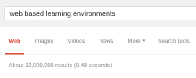
\includegraphics[]{minist-web}
    \caption{Căutare - tehnologii web}
    \label{fig:imag1}
\end{figure}

\begin{figure}[h, scale=2.0]
    \centering
    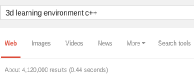
\includegraphics[]{minist-cpp}
    \caption{Căutare - tehnologii 3D și c++}
    \label{fig:imag2}
\end{figure}

\begin{table}
      \begin{center}
            \begin{tabular}{|l|l|l|}
                \hline 
                \cline{2-3}
                & $tehnologie$ & $pagini returnate$  \\ 
        	\hline
                $web$   &  32000000    &  0,48  \\
                $3D-C++$   &  4120000    &  0.44  \\
            \hline
	    \end{tabular}
        \end{center}
    \caption{Rezultate}
    \label{tab:rez}
\end{table}

\par Datele returnate de către motorul de căutare indică faptul că tehnologiile web sunt cu mult mai apreciate decât tehnologiile clasice cu grafică 3D, numărul de rezultate returnate fiind de 8 ori mai mare în favoarea tehnologiei web pentru timp de răspuns comparabil.